\documentclass{beamer}

\usepackage[frenchb]{babel}
\usepackage[T1]{fontenc}
\usepackage[utf8]{inputenc}
\usepackage{graphicx}

\usetheme{Warsaw}

\title{Réalisation d'un emploi du temps}
\author{Corentin Coudray - Christophe Julien - Nöel Tran}
\institute{ESME SUDRIA}

\begin{document}

\begin{frame}
\titlepage
\end{frame}

\section{Mise en forme des données}

\begin{frame}
Réalisation des emplois du temps par semestre

Un semestre est représenté par :
\begin{itemize}
\item Une liste de semaines
\item 22 créneaux de 2 heures par semaine
\end{itemize}
\end{frame}

\begin{frame}
5 fichiers d'informations : 
\begin{itemize}
\item Les professeurs
\item Les cours
\item Les classes
\item Les emplois du temps générés
\item La liste des cours non placés
\end{itemize}
\end{frame}

\subsection{Les professeurs}
\begin{frame} 
Les professeurs ont 4 informations : 
\begin{itemize}
\item l'identifiant
\item le nom
\item ses disponibilités
\item la liste des cours enseigné
\end{itemize}
\end{frame}

\begin{frame}
11 demi-journées par semaine\\
\vspace{\baselineskip}
Prof disponible  $\rightarrow$ 1\\
Prof non disponible  $\rightarrow$ 0\\
\vspace{\baselineskip}
Représentation des disponibilités d'un professeur sur les semaines:
\begin{itemize}
\item 1111 0011 1100 0011 1111 00
\end{itemize}
\end{frame}

\subsection{Les cours}
\begin{frame}
Les cours ont 3 informations : 
\begin{itemize}
\item l'identifiant
\item le nom
\item le nombre d'heure sur le semestre
\end{itemize}
\end{frame}

\subsection{Les classes}
\begin{frame}
Les classes ont 5 informations : 
\begin{itemize}
\item l'identifiant
\item le nom
\item la promotion à laquelle elle appartient
\item les cours à recevoir
\item le nombre d'élève
\end{itemize}
\end{frame}

\subsection{Les emplois du temps}
\begin {frame}
Chaque classe à 1 fichier d'emploi du temps.\\
Il contient pour chaque créneau : 
\begin {itemize}
\item l'identifiant du cours
\item l'identifiant du professeur
\end{itemize}
\end{frame}

\subsection{Les cours non placés}
\begin{frame}
Les cours qui n'ont pu être placé seront listés dans un fichier.
Chaque cours aura : 
\begin{itemize}
\item l'identifiant du cours
\item l'identifiant de la promotion
\item l'identifiant du professeur
\item le numéro de la semaine
\end{itemize}
\end{frame}

\section{Génération de l'emploi du temps}
\begin {frame}
Génération de l'emploi du temps à partir des fichiers d'entrés.

3 étapes de conception : 
\begin{itemize}
\item les pré-traitements
\item emploi du temps semestriel général
\item emploi du temps spécifique pour chaque classe
\end{itemize}
\end{frame}

\begin{frame}
Solution d'ordonnancement exacte difficile.\\
\vspace{\baselineskip}
Répartition aléatoire des cours sur les semaines\\
\vspace{\baselineskip}
Répartition des cours effectué sur un certain nombre d'itération
\end{frame}

\subsection{Pré-traitements}
\begin{frame}
Pré-traitement pour vérifier qu'une solution est potentiellement possible\\
\vspace{\baselineskip}
Evalutions du
\begin {itemize}
\item nombre de professeur
\item nombre d'heure de cours par promotion
\end{itemize}
\end{frame}

\begin{frame}
Nombre de professeurs suffisant pour donner l'ensemble des cours?
\end{frame}

\begin{frame}
Pour chaque cours de 2 heures : 
\begin{center}
$\sum_{i=0}^n dispo_{prof_i} > m$\\
\end{center}
\vspace{\baselineskip}
Pour chaque cours de 4 heures : \\
\begin{center}
$\frac{\sum_{i=0}^n dispo_{prof_i}}{2} > m$
\end{center}
\end{frame}

\begin{frame}
Le nombre d'heure de cours par promotion est supportable pour le semestre?
\end{frame}

\begin{frame}
\begin{center}
$\sum_{i=0}^n nbHeures_{cours_i} \leq s*c*h$
\end{center}
\begin{itemize}
\item $n$ le nombre de cours d'une classe $p$
\item $s$ le nombre de semaines sur un semestre
\item $c$ le nombre de créneaux sur une semaine 
\item $h$ le nombre d'heures d'un créneau
\end{itemize}
\end{frame}


\subsection{Emploi du temps semestriel}
\begin{frame}
Pour chaque promotion \\
\vspace{\baselineskip}
Objectif : \\
Répartir au mieux les cours sur le semestre\\
\vspace{\baselineskip}
Méthode : \\
Mettre le maximum de cours les uns derrière les autres
\end{frame}

\begin{frame}
Séparation des cours de 2 heures et 4 heures\\
\vspace{\baselineskip}
Tri en fonction du nombre de semaines\\
\vspace{\baselineskip}
Regroupement des 2 listes en une seule : \\
Première partie $\rightarrow$ cours de 4 heures triés\\
Seconde partie $\rightarrow$ cours de 2 heures triés
\end{frame}

\begin{frame}
Mise en place des répartitions des cours sur le semestre
\begin{center}
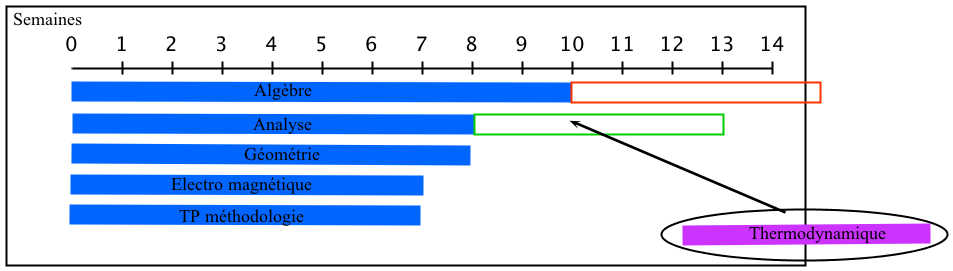
\includegraphics [width=117mm, height=60mm]{RepartitionSemestre2.png}
\end{center}
\end{frame}

\begin{frame}
Emploi du temps semestriel
\begin{center}
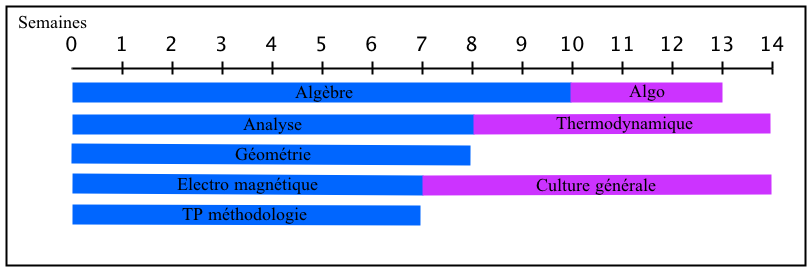
\includegraphics [width=110mm, height=60mm]{RepartitionSemestre.png}
\end{center}
\end{frame}

\subsection{Emploi du temps final}
\begin{frame}

\end{frame}





\end{document}